\section{The Implementation: The Search Process}
\label{sec:pit}

Now that we have discussed all the theoretical components of the search engine, it is time to move on to the actual implementation. In this section we describe in detail how a search query is processed and how it is presented to the end user.

\subsection{Entering A Query And Getting Results}

As to give an overview of what exactly happens during a typical search, we will show what happens during a normal search process. From the user perspective, everything happens inside a web browser. When the user visits the demo page \cite{self:sqesdemo}, they are presented with a frontend as shown in Figure \ref{fig:frontmain}.

\begin{figure}[h]
  \begin{center}
    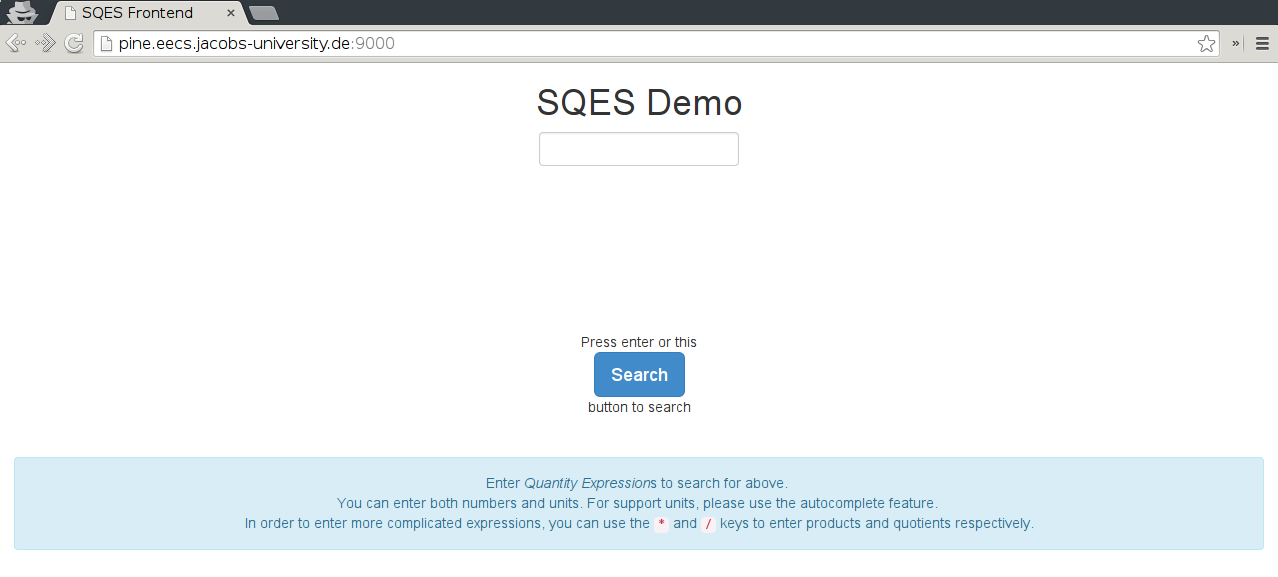
\includegraphics[width=\textwidth]{img/screen1.png}
  \end{center}
  \caption{The main page of the frontend. }
  \label{fig:frontmain}
\end{figure}

Because the frontend is running inside a Webbrowser it is written using HTML, CSS and JavaScript. Furthermore it uses the frameworks jQuery \cite{lib:jquery} and Bootstrap \cite{lib:bootstrap}. As seen in the figure, the main components are a text field to enter a quantity expression as well as a search button.

With the text field it is easily possible to enter composed quantity expression.

When searching for a certain unit it is neccessary to tell the backend which \textit{unit theory} this unit comes from. In order to make this easier, the GUI has an autocompletion feature. It is only required to enter the name of the unit itself and the possible theories this unit can come from will be suggested automatically.

Apart from entering a simple unit it is possible for the user to compose quantity expressions by multiplication and division. If the keys ``*'' and ``/'' are pressed, the text field splits into two different fields. In each of them another quantity expression can be entered.

In order to facilitate entering division and multiplication by numbers, it is also possible to enter numbers into these fields. With this input unit it is also possible to enter all the quantity expressions as described by the formalism above. In Figure \ref{fig:frontauto} the process of entering the query $42 \frac{\text{Furlong}}{\text{Fortnight}}$ is shown.

\begin{figure}
  \centering
  \begin{subfigure}[b]{0.9\textwidth}
          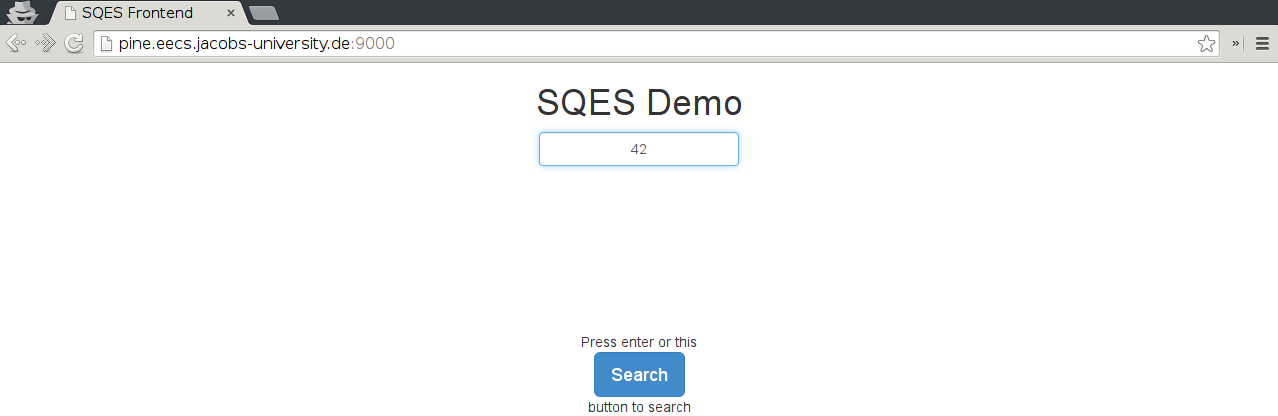
\includegraphics[width=\textwidth]{img/enter1}
          \caption{Entering a number}
          \label{fig:frontauto1}
  \end{subfigure}
  \\
  \begin{subfigure}[b]{0.9\textwidth}
          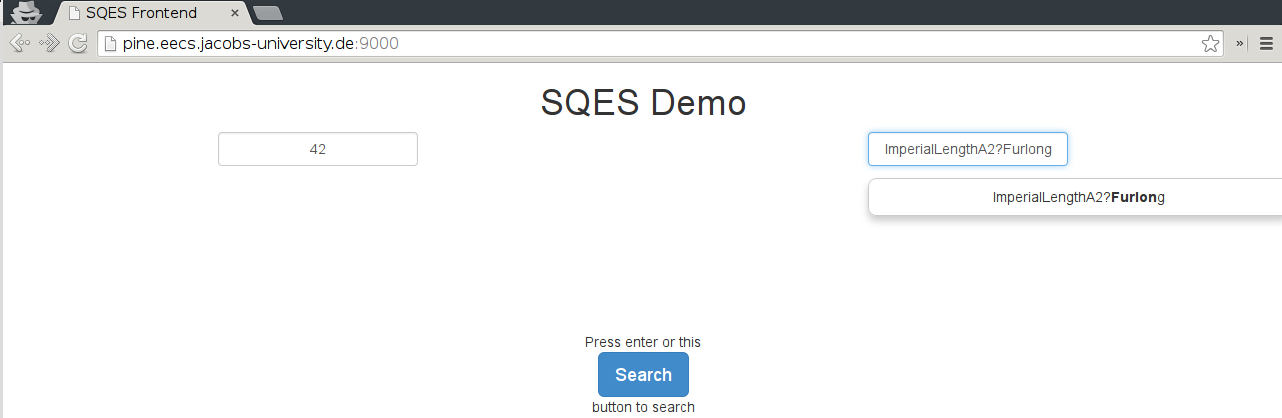
\includegraphics[width=\textwidth]{img/enter2}
          \caption{Entering and autocompleting the unit \textit{Furlong}}
          \label{fig:frontauto2}
  \end{subfigure}
  \\
  \begin{subfigure}[b]{0.9\textwidth}
          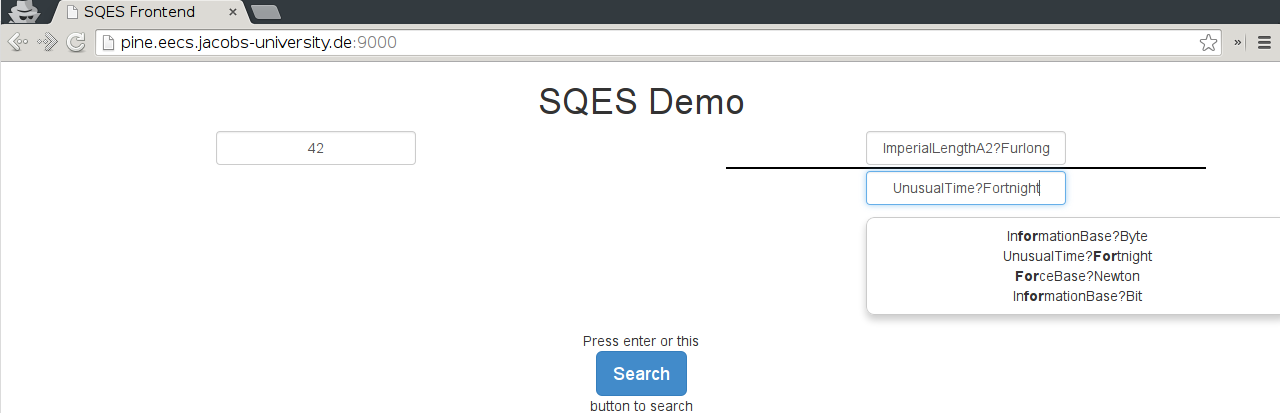
\includegraphics[width=\textwidth]{img/enter3}
          \caption{Entering the final component. }
          \label{fig:frontauto3}
  \end{subfigure}
  \caption{Process of entering the quantity expression $42 \frac{\text{Furlong}}{\text{Fortnight}}$ into the frontend. }
  \label{fig:frontauto}
\end{figure}

After the quantity expression has been entered, the search can be started by pressing the \textit{Search} button or hitting the \textit{Enter} key. Once the results have been received from the backend they are displayed to the user. The result page lists the found Quantity Expressions in their original forms\footnote{Currently they are only displayed as serialised XML, this is discussed in more detail in section \ref{sec:fut_res}. } and links to the locations where they were found inside the actual document in the spotter. An example can be found in Figure \ref{fig:frontres}.

\begin{figure}
  \begin{center}
    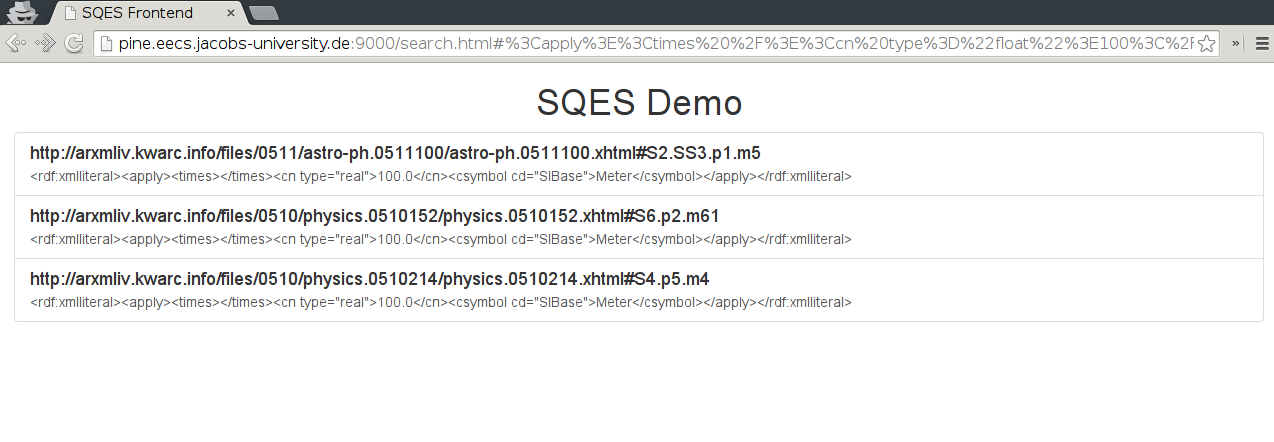
\includegraphics[width=\textwidth]{img/res1.png}
  \end{center}
  \caption{The result page when searching for $100$ Meters. }
  \label{fig:frontres}
\end{figure}

\subsection{Preparing The Backend}

After the query has been entered into the frontend, it is serialised to XML as shown in Section \ref{sec:xml}. This XML is then sent to the backend.

The backend is written in Scala and exposes its functionality via HTTP. Before the backend is ready to receive queries, it has to normalise the quantity expressions found by the Spotter. These queries are also provided in XML form. This XML is parsed and deserialised into an internal data structure.

Next we want to normalise these quantity expressions using the algorithm described in Section \ref{sec:norm}. In order to achieve this the backend first parses the MMT theories and views and builds up a theory graph. Next, it normalises all units found inside the unit graph and caches these normal forms in memory.

We can then use the forms to quickly normalise all the quantity expression found inside the harvests. The normalised forms are then used to store them in an appropriate structure on disk. In this structure all equivalent quantity expressions are stored inside the same folder. This allows very quick access to all quantity expressions in preparation for processing a query.

\subsection{Processing A Typical Query}

Upon receiving the query, the backend deserialises and normalises the XML as it did for all the harvests. Since the normal forms of each \textit{basic unit} are still cached inside memory, this process is very quick. Because the normal forms are already cached on disk, the process of finding equivalent quantity expressions can be efficiently done. As described above, all equivalent quantity expressions are in the same folder. The backend now just reads all the quantity expressions stored inside the folder the query falls in. This delivers all equivalent quantity expressions and can be sent back the frontend.

Because all the normal forms are simply stored on disk inside a folder it is easily possible to add more quantity expressions to an existing harvest. This is even possible during query timee. For this reason the implementation of the search engine has two seperate modes, a \textit{harvest} mode and a \textit{query} mode which allow preprocessing of harvests and actual querying. Since the first mode does not require network interaction, only the query mode has an actual HTTP interface.
